\documentclass[aspectratio=43]{beamer}

% Title --------------------------------------------
\title{\huge Wartime violence}
\author{Francisco Villamil}
\date{War, peace, and political violence\\UC3M, Fall 2023}

%%% NOTE -- CHECK THIS: https://github.com/paulgp/beamer-tips


%%% Building heavily on https://github.com/kylebutts/templates

% xcolor, define them
\usepackage{xcolor}

% TEXT COLORS
\definecolor{red}{HTML}{9a2515}
\definecolor{yellow}{HTML}{EBC944}
\definecolor{asher}{HTML}{555F61}
\definecolor{jet}{HTML}{131516}

% THEME COLORS
\definecolor{accent}{HTML}{107895}
\definecolor{accent2}{HTML}{9a2515}

% Color commands
\newcommand\red[1]{{\color{red}#1}}
\newcommand\yellow[1]{{\color{yellow}#1}}
\newcommand\asher[1]{{\color{asher}#1}}

\newcommand\BGred[1]{{\colorbox{red!80!white}{#1}}}
\newcommand\BGyellow[1]{{\colorbox{yellow!80!white}{#1}}}
\newcommand\BGasher[1]{{\colorbox{asher!80!white}{#1}}}

\renewcommand<>{\BGyellow}[1]{\only#2{\beameroriginal{\BGyellow}}{#1}}

% Appendix numbering
\usepackage{appendixnumberbeamer}

% Beamer Options -------------------------------------

% Background
\setbeamercolor{background canvas}{bg = white}

% Change text margins
\setbeamersize{text margin left = 25pt, text margin right = 15pt}

% \alert
\setbeamercolor{alerted text}{fg = accent2}

% Frame title
\setbeamercolor{frametitle}{bg = white, fg = jet}
\setbeamercolor{framesubtitle}{bg = white, fg = accent}
\setbeamerfont{framesubtitle}{size = \small, shape = \itshape}

% Block
\setbeamercolor{block title}{fg = white, bg = accent2}
\setbeamercolor{block body}{fg = jet, bg = jet!10!white}

% Title page
\setbeamercolor{title}{fg = jet}
\setbeamercolor{subtitle}{fg = accent}

%% Custom \maketitle and \titlepage
\setbeamertemplate{title page}
{
    \begin{centering}
      % \vspace{20mm}
      {\Large \usebeamerfont{title}\usebeamercolor[fg]{title}\inserttitle}\\ \vskip0.25em%
      \ifx\insertsubtitle\@empty%
      \else%
        {\usebeamerfont{subtitle}\usebeamercolor[fg]{subtitle}\insertsubtitle\par}%
      \fi%
      {\vspace{10mm}\insertauthor}\\
      \ifx\insertinstitute\@empty%
      \else%
        {\vspace{5mm}\color{asher}\scriptsize{\insertinstitute}}
      \fi%
      {\color{asher}\small{\insertdate}}\\
    \end{centering}
}

% Table of Contents
\setbeamercolor{section in toc}{fg = accent!70!jet}
\setbeamercolor{subsection in toc}{fg = jet}

% Button
\setbeamercolor{button}{bg = accent}

% Remove navigation symbols
\setbeamertemplate{navigation symbols}{}

% Table and Figure captions
\setbeamercolor{caption}{fg=jet!70!white}
\setbeamercolor{caption name}{fg=jet}
\setbeamerfont{caption name}{shape = \itshape}

% Put slide number / total slides at the bottom right
\makeatother
\makeatletter
\setbeamertemplate{footline} %{\hfill\insertframenumber/\inserttotalframenumber}
{%
  \leavevmode%
  \hbox{
  \begin{beamercolorbox}[wd=\paperwidth,ht=2.5ex,dp=1.125ex,leftskip=.3cm,rightskip=.3cm plus1fil]{footlinecolor}%
    \color{asher}{\hfill\insertframenumber/\inserttotalframenumber}
  \end{beamercolorbox}}%
  \vskip0pt%
}
\makeatother
\makeatletter

% Bullet points

%% Fix left-margins
\settowidth{\leftmargini}{\usebeamertemplate{itemize item}}
\addtolength{\leftmargini}{\labelsep}

%% enumerate item color
\setbeamercolor{enumerate item}{fg = accent}
\setbeamerfont{enumerate item}{size = \small}
\setbeamertemplate{enumerate item}{\insertenumlabel.}

%% itemize
\setbeamercolor{itemize item}{fg = accent!70!white}
\setbeamerfont{itemize item}{size = \small}
\setbeamertemplate{itemize item}[circle]
\setlength{\itemsep}{0pt plus 6pt}

%% right arrow for subitems
\setbeamercolor{itemize subitem}{fg = accent!60!white}
\setbeamerfont{itemize subitem}{size = \small}
\setbeamertemplate{itemize subitem}{$\rightarrow$}

\setbeamertemplate{itemize subsubitem}[square]
\setbeamercolor{itemize subsubitem}{fg = jet}
\setbeamerfont{itemize subsubitem}{size = \small}

% References

%% Bibliography Font, roughly matching aea
\setbeamerfont{bibliography item}{size = \footnotesize}
\setbeamerfont{bibliography entry author}{size = \footnotesize, series = \bfseries}
\setbeamerfont{bibliography entry title}{size = \footnotesize}
\setbeamerfont{bibliography entry location}{size = \footnotesize, shape = \itshape}
\setbeamerfont{bibliography entry note}{size = \footnotesize}

\setbeamercolor{bibliography item}{fg = jet}
\setbeamercolor{bibliography entry author}{fg = accent!60!jet}
\setbeamercolor{bibliography entry title}{fg = jet}
\setbeamercolor{bibliography entry location}{fg = jet}
\setbeamercolor{bibliography entry note}{fg = jet}

%% Remove bibliography symbol in slides
\setbeamertemplate{bibliography item}{}





% Links ----------------------------------------------

\usepackage{hyperref}
\hypersetup{
  colorlinks = true,
  linkcolor = accent,
  filecolor = accent,
  urlcolor = accent,
  citecolor = accent,
}


% Line spacing --------------------------------------
\usepackage{setspace}
\setstretch{1.2}


% \begin{columns} -----------------------------------
\usepackage{multicol}


% % Fonts ---------------------------------------------
% % Beamer Option to use custom fonts
% \usefonttheme{professionalfonts}
%
% % \usepackage[utopia, smallerops, varg]{newtxmath}
% % \usepackage{utopia}
% \usepackage[sfdefault,light]{roboto}
%
% % Small adjustments to text kerning
% \usepackage{microtype}



% Remove annoying over-full box warnings -----------
\vfuzz2pt
\hfuzz2pt


% Table of Contents with Sections
\setbeamerfont{myTOC}{series=\bfseries, size=\Large}
\AtBeginSection[]{
        \frame{
            \frametitle{Roadmap}
            \tableofcontents[current]
        }
    }


% References ----------------------------------------
\usepackage[
    citestyle= authoryear,
    style = authoryear,
    natbib = true,
    backend = biber
]{biblatex}

% Smaller font-size for references
\renewcommand*{\bibfont}{\small}

% Remove "In:"
\renewbibmacro{in:}{}

% Color citations for slides
\newenvironment{citecolor}
    {\footnotesize\begin{color}{accent2}}
    {\end{color}}

\newcommand{\citetcolor}[1]{{\footnotesize\textcolor{asher}{\citet{#1}}}}
\newcommand{\citepcolor}[1]{{\footnotesize\textcolor{asher}{\citep{#1}}}}

% Tables -------------------------------------------
% Tables too big
% \begin{adjustbox}{width = 1.2\textwidth, center}
\usepackage{adjustbox}
\usepackage{array}
\usepackage{threeparttable, booktabs, adjustbox}

% Fix \input with tables
% \input fails when \\ is at end of external .tex file

\makeatletter
\let\input\@@input
\makeatother

% Tables too narrow
% \begin{tabularx}{\linewidth}{cols}
% col-types: X - center, L - left, R -right
% Relative scale: >{\hsize=.8\hsize}X/L/R
\usepackage{tabularx}
\newcolumntype{L}{>{\raggedright\arraybackslash}X}
\newcolumntype{R}{>{\raggedleft\arraybackslash}X}
\newcolumntype{C}{>{\centering\arraybackslash}X}

% Figures

% \imageframe{img_name} -----------------------------
% from https://github.com/mattjetwell/cousteau
\newcommand{\imageframe}[1]{%
    \begin{frame}[plain]
        \begin{tikzpicture}[remember picture, overlay]
            \node[at = (current page.center), xshift = 0cm] (cover) {%
                \includegraphics[keepaspectratio, width=\paperwidth, height=\paperheight]{#1}
            };
        \end{tikzpicture}
    \end{frame}%
}

% subfigures
\usepackage{subfigure}


% Highlight slide -----------------------------------
% \begin{transitionframe} Text \end{transitionframe}
% from paulgp's beamer tips
\newenvironment{transitionframe}{
    \setbeamercolor{background canvas}{bg=accent!60!black}
    \begin{frame}\color{accent!10!white}\LARGE\centering
}{
    \end{frame}
}


% Table Highlighting --------------------------------
% Create top-left and bottom-right markets in tabular cells with a unique matching id and these commands will outline those cells
\usepackage[beamer,customcolors]{hf-tikz}
\usetikzlibrary{calc}
\usetikzlibrary{fit,shapes.misc}

% To set the hypothesis highlighting boxes red.
\newcommand\marktopleft[1]{%
    \tikz[overlay,remember picture]
        \node (marker-#1-a) at (0,1.5ex) {};%
}
\newcommand\markbottomright[1]{%
    \tikz[overlay,remember picture]
        \node (marker-#1-b) at (0,0) {};%
    \tikz[accent!80!jet, ultra thick, overlay, remember picture, inner sep=4pt]
        \node[draw, rectangle, fit=(marker-#1-a.center) (marker-#1-b.center)] {};%
}



\begin{document}

\begin{frame}
  \titlepage
\end{frame}


% ----------------------------------------------------
\imageframe{img/gaza1}
% ----------------------------------------------------

% ----------------------------------------------------
\imageframe{img/gaza2}
% ----------------------------------------------------

% ----------------------------------------------------
\imageframe{img/gaza3}
% ----------------------------------------------------

% ----------------------------------------------------
\begin{frame}
\frametitle{Key question}
\centering

\begin{itemize}[<+->]
  \item \textbf{Why do civilians die in a war?}
  \item And how does this vary?
  \begin{itemize}
    \item across \BGyellow<3>{conflicts}?
    \item across \BGyellow<4>{actors}?
    \item across \BGyellow<5>{time}?
    \item across \BGyellow<6>{space}?
  \end{itemize}
  \item We can also ask the same about \textbf{battle violence}
\end{itemize}



\end{frame}
% ----------------------------------------------------

% ----------------------------------------------------
\begin{frame}
\frametitle{What we have seen so far}
\centering

\begin{itemize}
  \item<1-> Focus on whole conflicts/events
  \begin{itemize}
    \item WWII, Sri Lankan Civil War, Israel-Gaza conflict, etc
  \end{itemize}
  \item<2-> Historical trends in conflicts and big global changes
  \begin{itemize}
    \item What historical events explain long-term trends in war?
  \end{itemize}
  \item<3-> Causes of individual conflicts
  \begin{itemize}
    \item Why did e.g. the Second Congo War break out? What countries are at risk of conflict?
  \end{itemize}
\end{itemize}

\end{frame}
% ----------------------------------------------------

% ----------------------------------------------------
\begin{frame}<1-7>[label=previous]
\frametitle{What we have seen so far}
\centering

\begin{itemize}[<+->]
  \item But we're also very interested in patterns of \BGyellow{violence}
  \begin{itemize}
    \item which varies a lot
    \item we can talk about several types: battle violence, \textbf{violence against civilians}, intentional vs collateral, fatal vs non-fatal, ...
  \end{itemize}
  \item Some people don't pay much attention to this: they are just interested in the causes of conflicts
  \begin{itemize}
    \item In civil wars, violence is assumed to be more brutal and involve civilians more often
    \item In inter-state war studies, many just used to define a minimum of \textit{battle deaths} to call a war a war, and then just ignore it (which also sidelines other forms of violence, such as violence against civilians)
  \end{itemize}
  \item But just think about WWII for a second
  \item Violence \textit{varies} and is \textit{not random} at all
\end{itemize}

\end{frame}
% ----------------------------------------------------

% ----------------------------------------------------
\begin{frame}
\frametitle{Violence patterns during WWII}
\centering

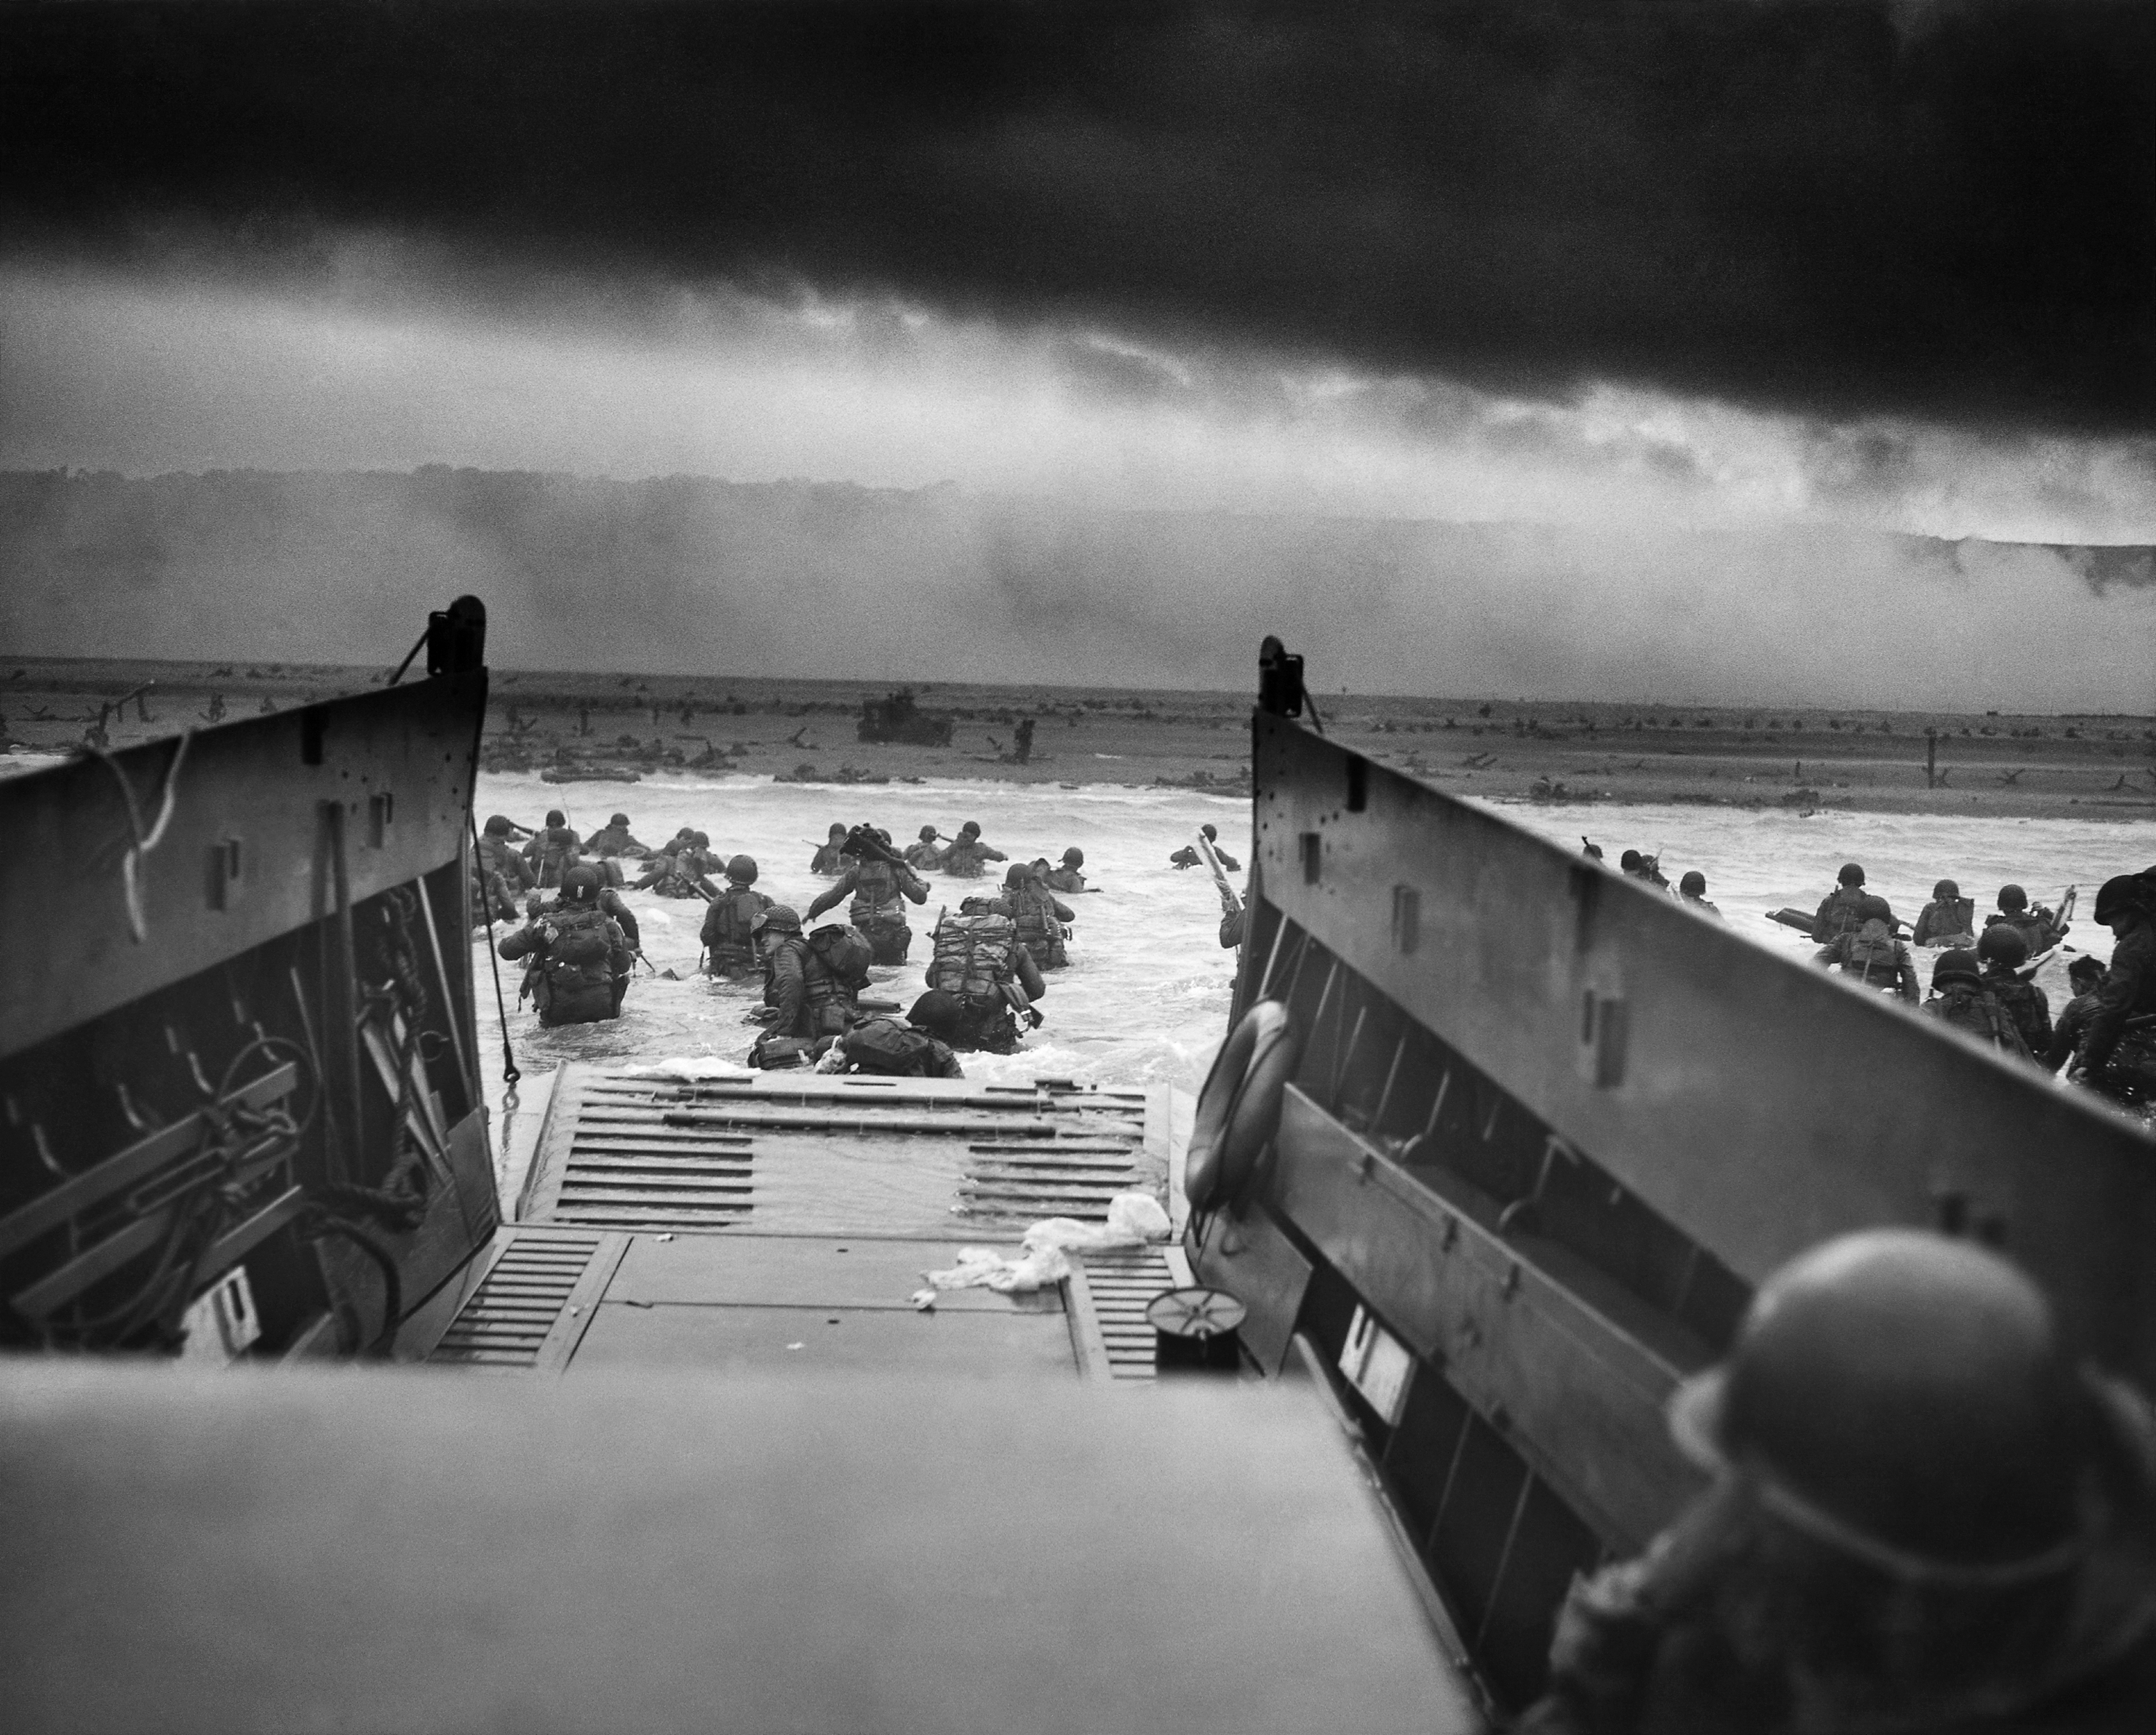
\includegraphics[width = 0.8\textwidth]{img/wwii-normandy}

Battle of Normandy

\end{frame}
% ----------------------------------------------------

% ----------------------------------------------------
\begin{frame}
\frametitle{Violence patterns during WWII}
\centering

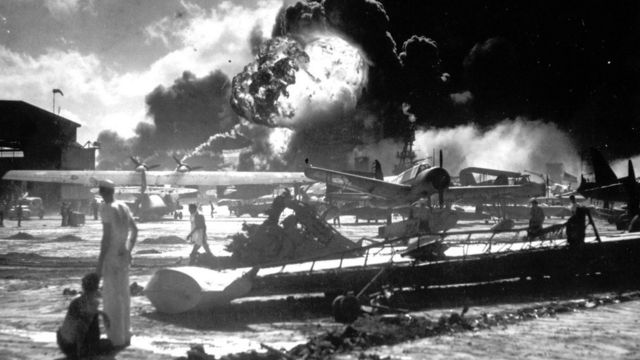
\includegraphics[width = 0.8\textwidth]{img/wwii-pearlharbor}

Pearl Harbor

\end{frame}
% ----------------------------------------------------

% ----------------------------------------------------
\begin{frame}
\frametitle{Violence patterns during WWII}
\centering

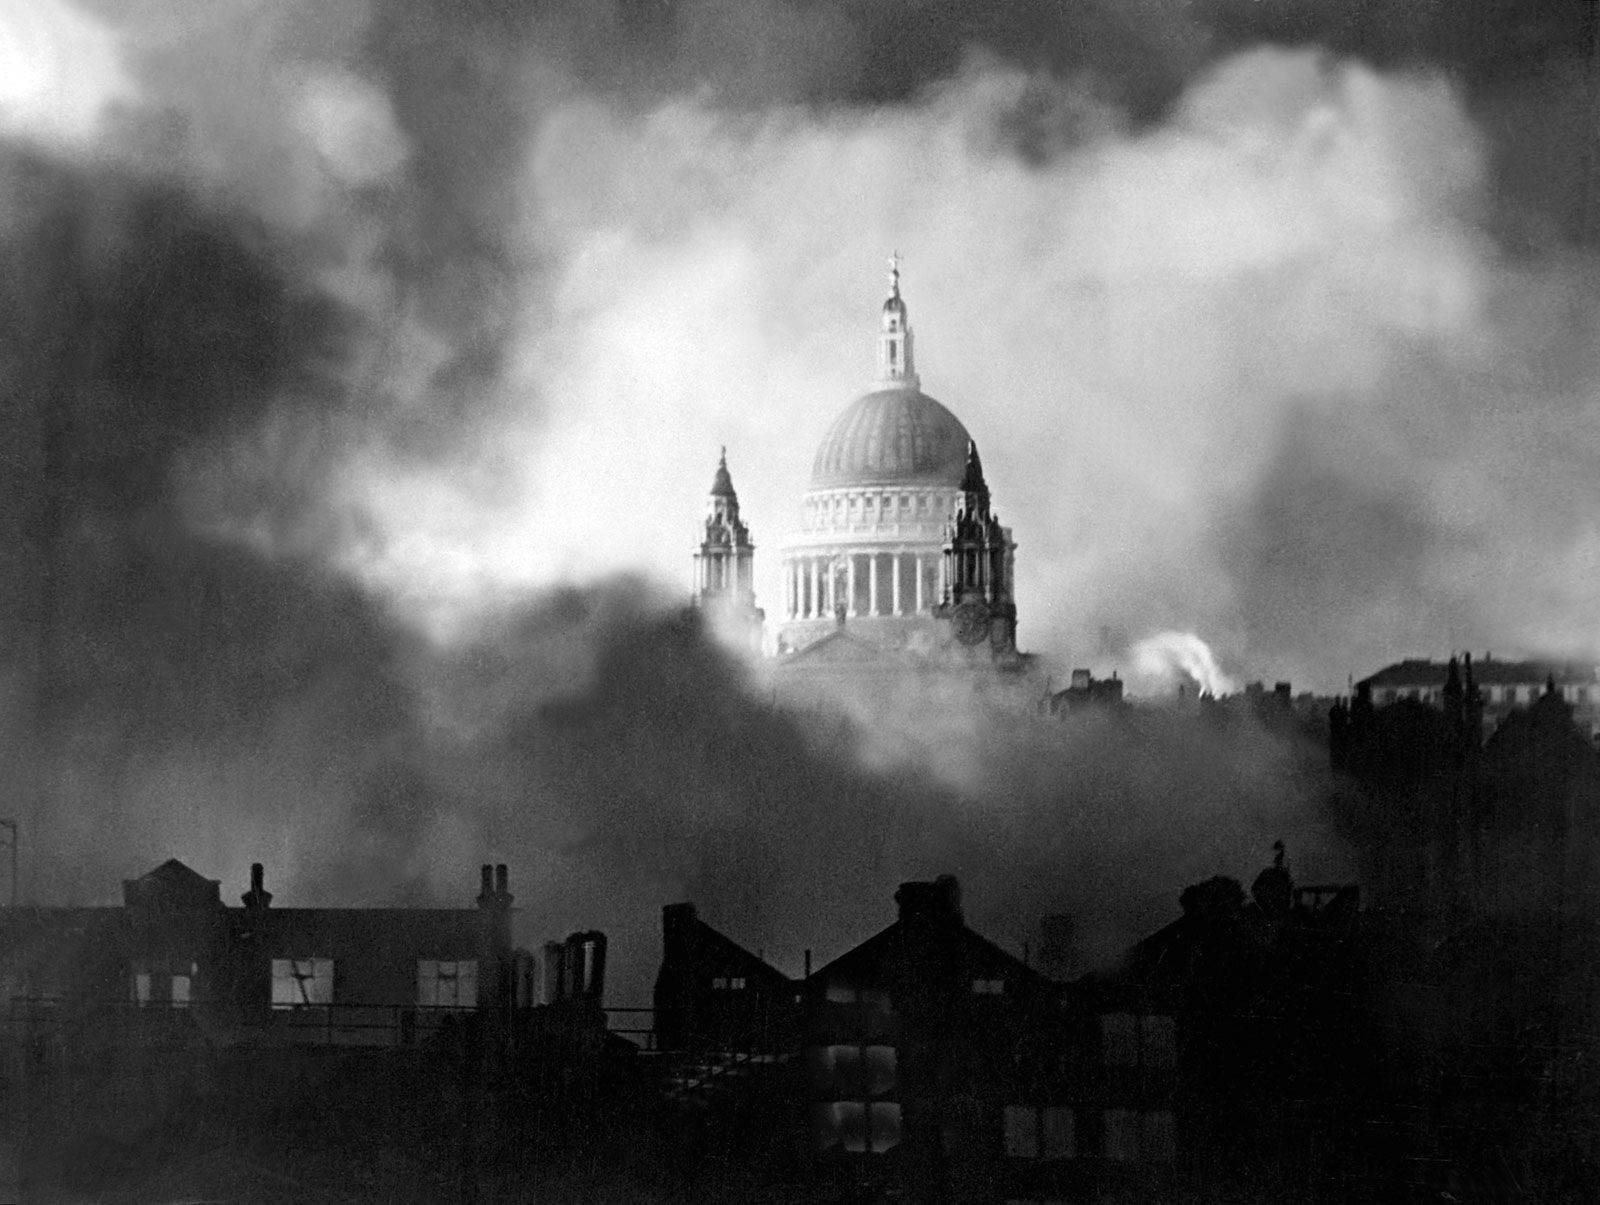
\includegraphics[width = 0.8\textwidth]{img/wwii-londonblitz}

London Blitz

\end{frame}
% ----------------------------------------------------

% ----------------------------------------------------
\begin{frame}
\frametitle{Violence patterns during WWII}
\centering

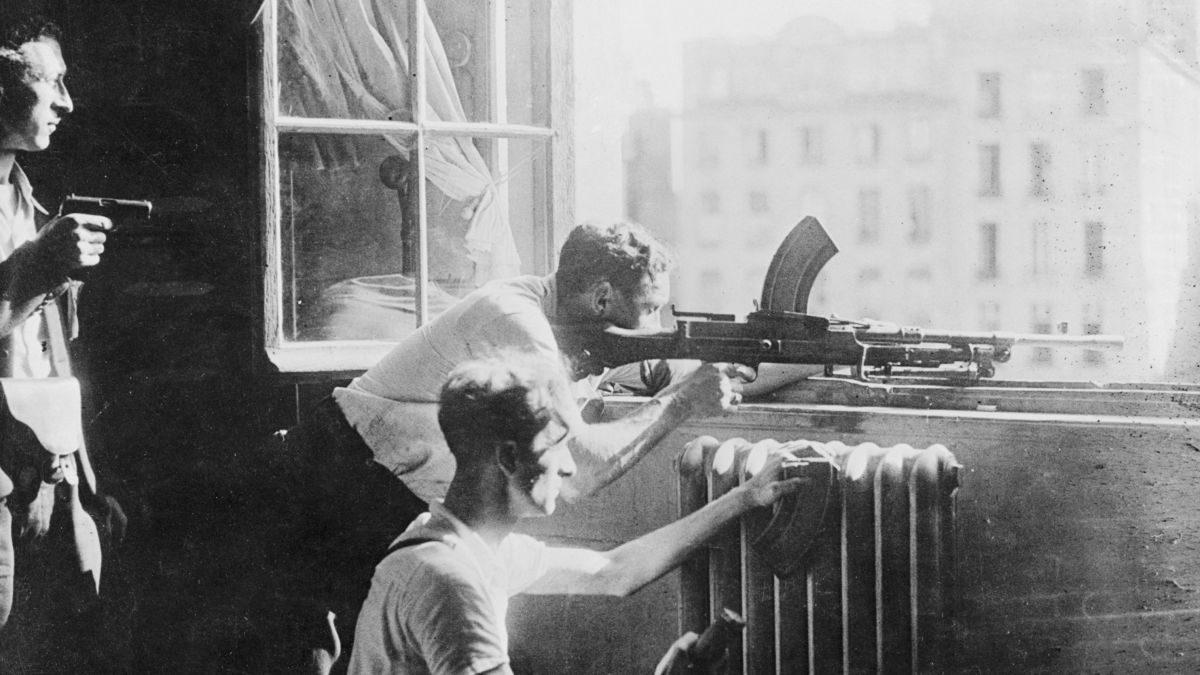
\includegraphics[width = 0.8\textwidth]{img/wwii-resistance}

French Resistance

\end{frame}
% ----------------------------------------------------

% ----------------------------------------------------
\begin{frame}
\frametitle{Violence patterns during WWII}
\centering

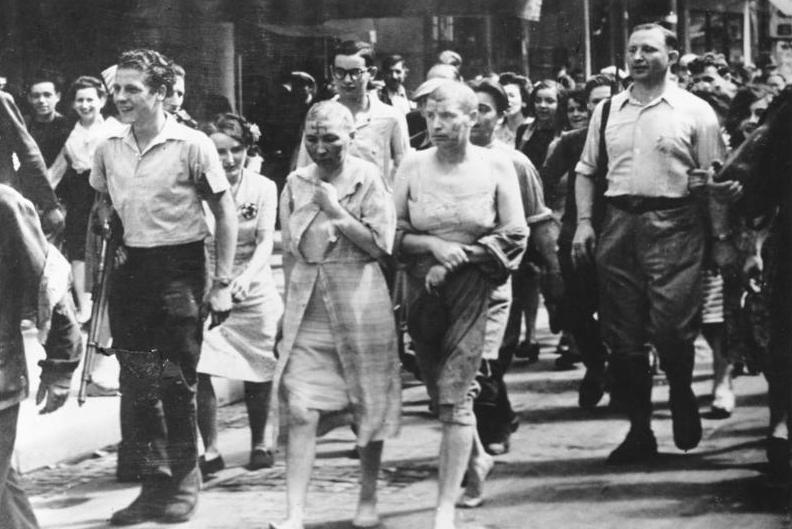
\includegraphics[width = 0.8\textwidth]{img/wwii-womencolab}

Women accused of collaboration with the Nazis, Paris 1944

\end{frame}
% ----------------------------------------------------

% ----------------------------------------------------
\begin{frame}
\frametitle{Violence patterns during WWII}
\centering

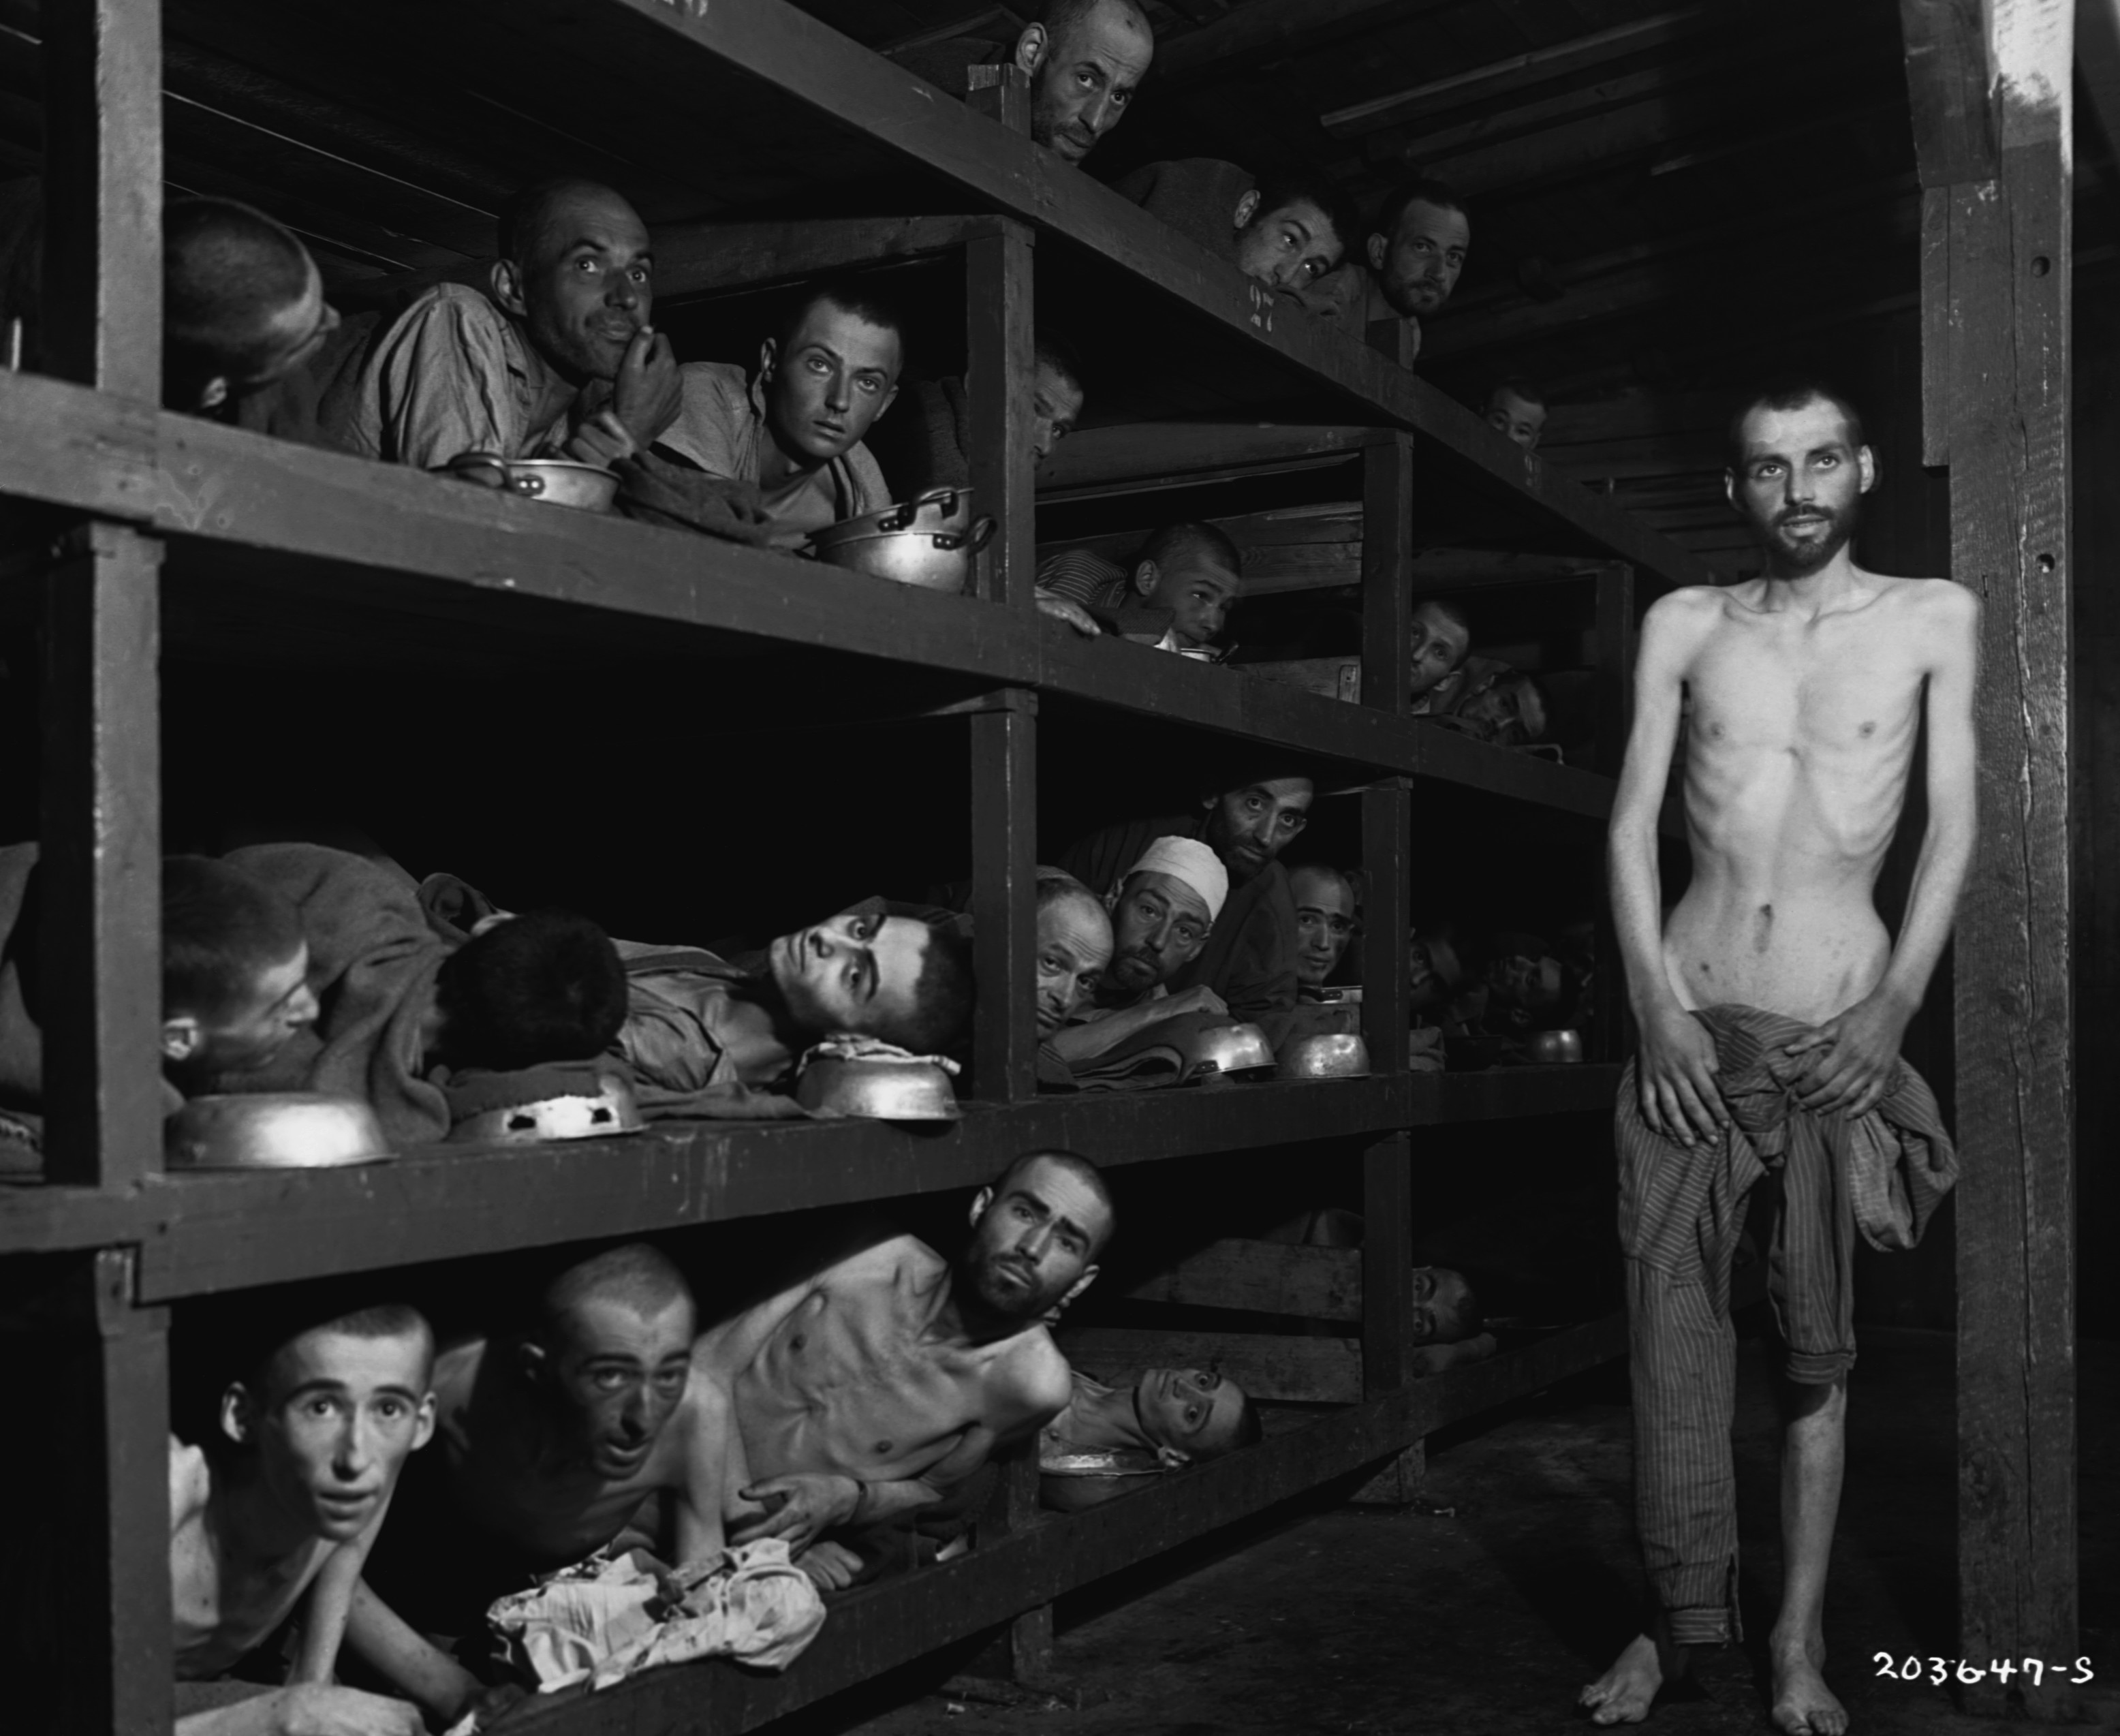
\includegraphics[width = 0.8\textwidth]{img/wwii-holocaust}

Holocaust against Jews

\end{frame}
% ----------------------------------------------------

% ----------------------------------------------------
\begin{frame}
\frametitle{Violence patterns during WWII}
\centering

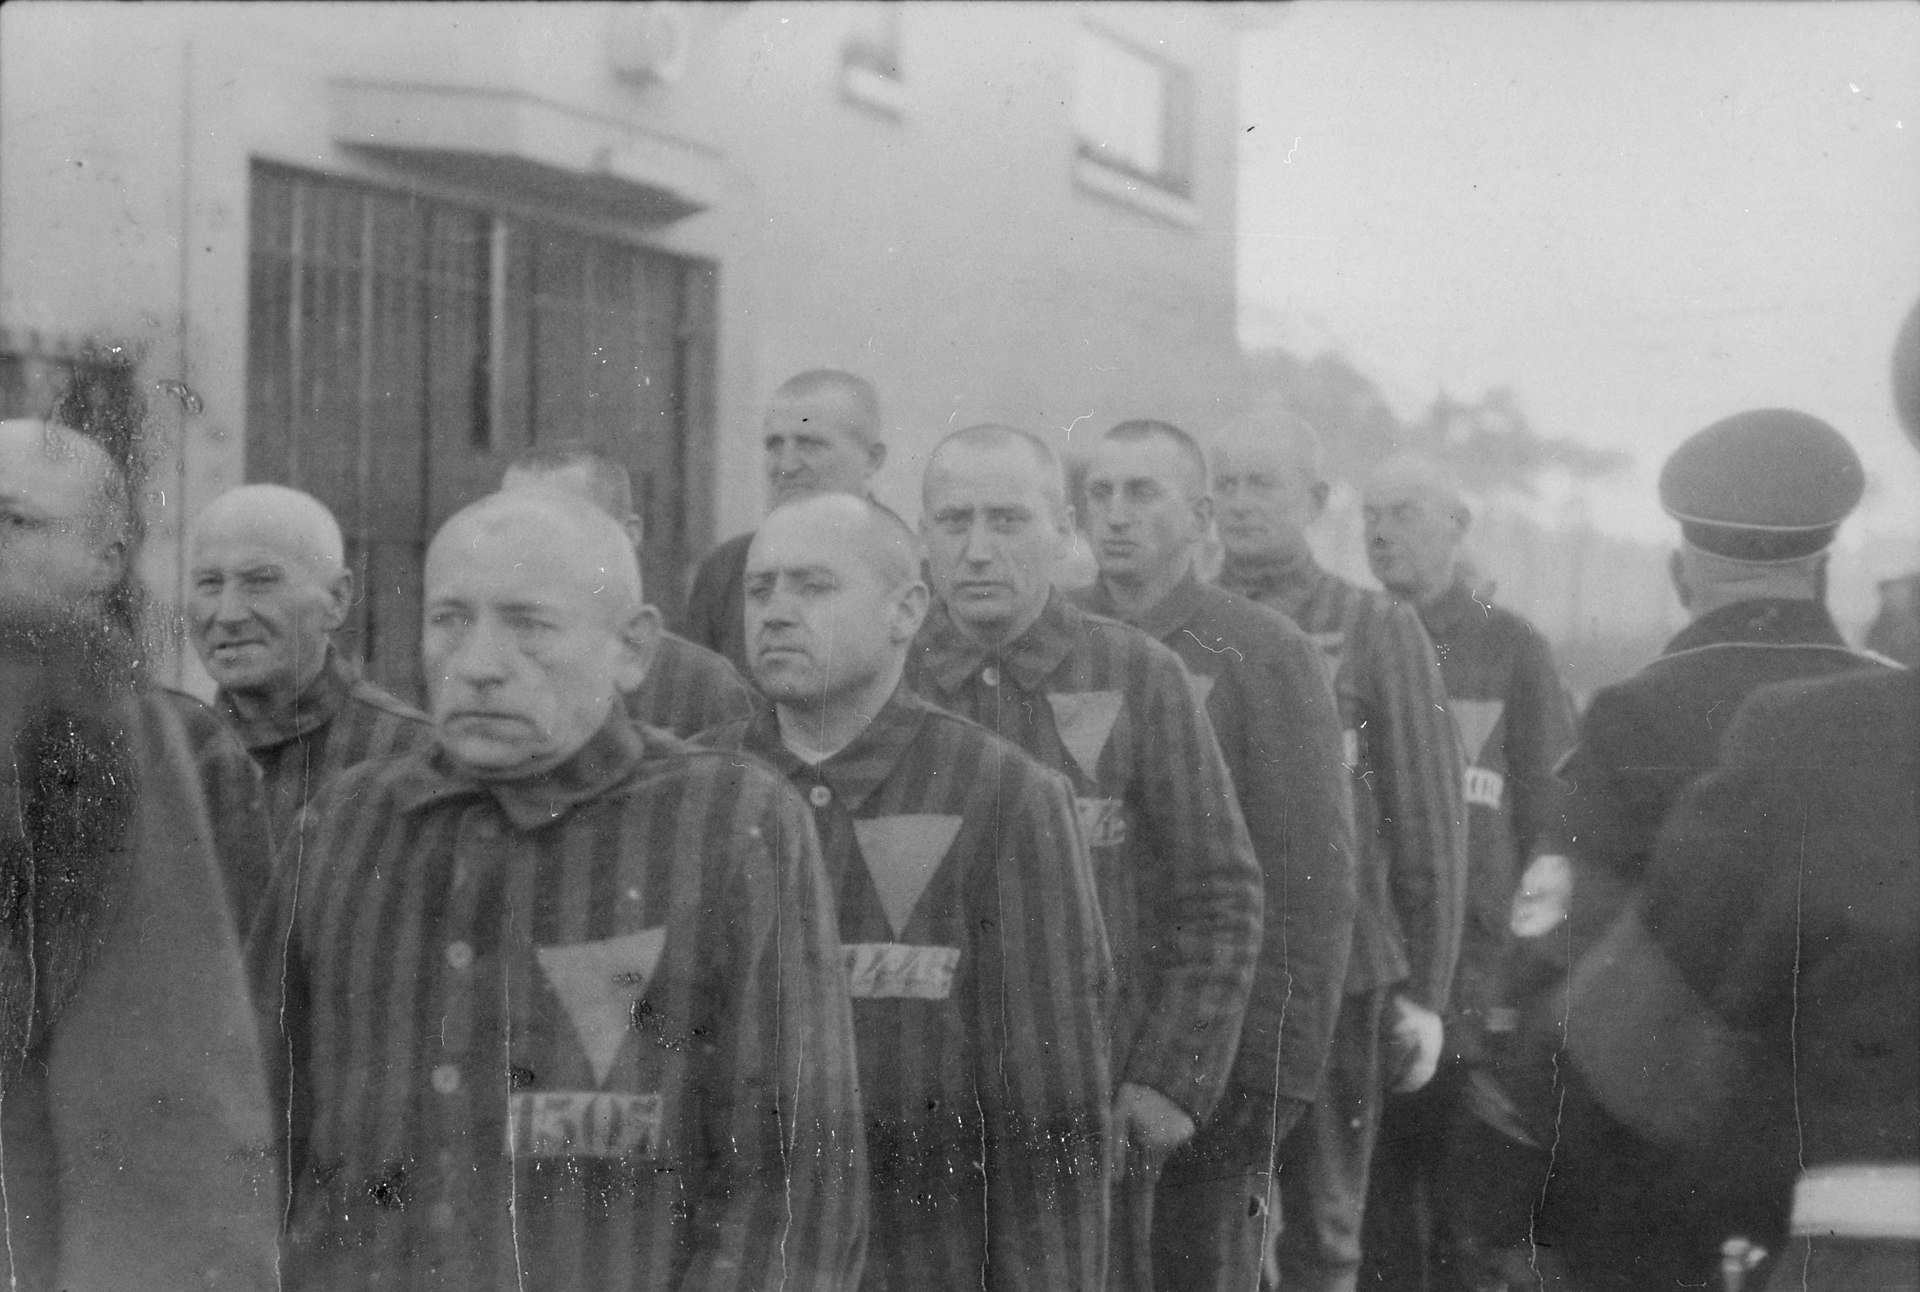
\includegraphics[width = 0.8\textwidth]{img/wwii-Sachsenhausen}

Political prisoners in Sachsenhausen camp

\end{frame}
% ----------------------------------------------------

% ----------------------------------------------------
\againframe<5-6>{previous}
% ----------------------------------------------------

% ----------------------------------------------------
\begin{frame}
\frametitle{Violence in civil wars}
\centering

\begin{itemize}
  \item<1-> Even more relevant when talking about civil wars, because the role of civilians is subtantially different
  \begin{itemize}
    \item<2-> military contest vs barbarian chaos, battle for hearts and minds, ...
  \end{itemize}
  \item<3-> Key aspect: distinction between \BGyellow{battle violence} and \BGyellow{violence against civilians}
  \begin{itemize}
    \item Blurry in civil wars: what distinguishes a combatant from a civilian?
    \item Compare with idea of civilians in interstate wars and \textit{jus in bello} (IHL)
  \end{itemize}
\end{itemize}

\end{frame}
% ----------------------------------------------------

% ----------------------------------------------------
\begin{frame}
\frametitle{Violence in civil wars}
\centering

\begin{itemize}
  \item We are going to talk a lot about two (or three) important things relatively unique to civil wars
  \item<2->[1.] \BGyellow{Role of civilians in civil wars}
  \begin{itemize}
    \item `Object' of fighting (a civil war is a war over sovereignty, political rule needs some support, etc), role of support and obedience, etc
  \end{itemize}
  \item<3->[2.] \BGyellow{Problem of information}
  \begin{itemize}
    \item Not for us to distinguish battle violence, but for combatants: who's the enemy?
  \end{itemize}
  \item<4->[(*)] `Informality' of civil wars (less rules, less hierarchy, less central planning)
\end{itemize}

\end{frame}
% ----------------------------------------------------

% ----------------------------------------------------
\begin{frame}
\frametitle{Types of violence}
\centering

\begin{itemize}
  \item<1->[] According to whether they are armed actors or not:
  \item<2-> Battle violence (or bilateral)
  \item<2-> \BGyellow<3->{Violence against civilians} (or unilateral)
  \begin{itemize}
    \item<3-> We'll focus on this: violence by armed organizations against unarmed civilians
    \item<3-> Very relevant in the context of civil wars
    \item<3-> Usually the source of war-related suffering, many consequences, legally sanctioned...
  \end{itemize}
  \item[]
  \item<4-> Sometimes: state-based, non-state, one-sided
  \item<5-> \textbf{What's the difference between state-based violence and state-based conflicts?}
\end{itemize}

\end{frame}
% ----------------------------------------------------

% ----------------------------------------------------
\begin{frame}
\frametitle{Types of violence}
\centering

\begin{itemize}[<+->]
  \item This distinction is based on the actors who perpetrate violence and who are the target of violence
  \item But when we look at how violence is \textit{used}, there is a lot of variation
\end{itemize}


\end{frame}
% ----------------------------------------------------

% ----------------------------------------------------
\begin{frame}
\frametitle{Patterns of political violence \hfill {\scriptsize (Gutierrez-Sanín \& Wood 2017)}}
\centering

% \begin{itemize}
%   \item We can use a more nuanced description of the pattern of political violence, usually referred to an organization (Gutierrez-Sanín \& Wood, 2017)
%   \item Repertoire
%   \begin{itemize}
%     \item Forms of violence usually employed: homicide, torture, displacement, rape...
%   \end{itemize}
%   \item Targeting
%   \begin{itemize}
%     \item Which social group is directed at? Selective violence, collective violence, `indiscriminate' violence, etc
%   \end{itemize}
%   \item Technique
%   \begin{itemize}
%     \item Method used to commit violence: small firearms, machetes, aerial bombings, suicide bombing, etc
%   \end{itemize}
%   \item Frequency
%   \begin{itemize}
%     \item Count of violent events, or rate or incidence
%   \end{itemize}
% \end{itemize}

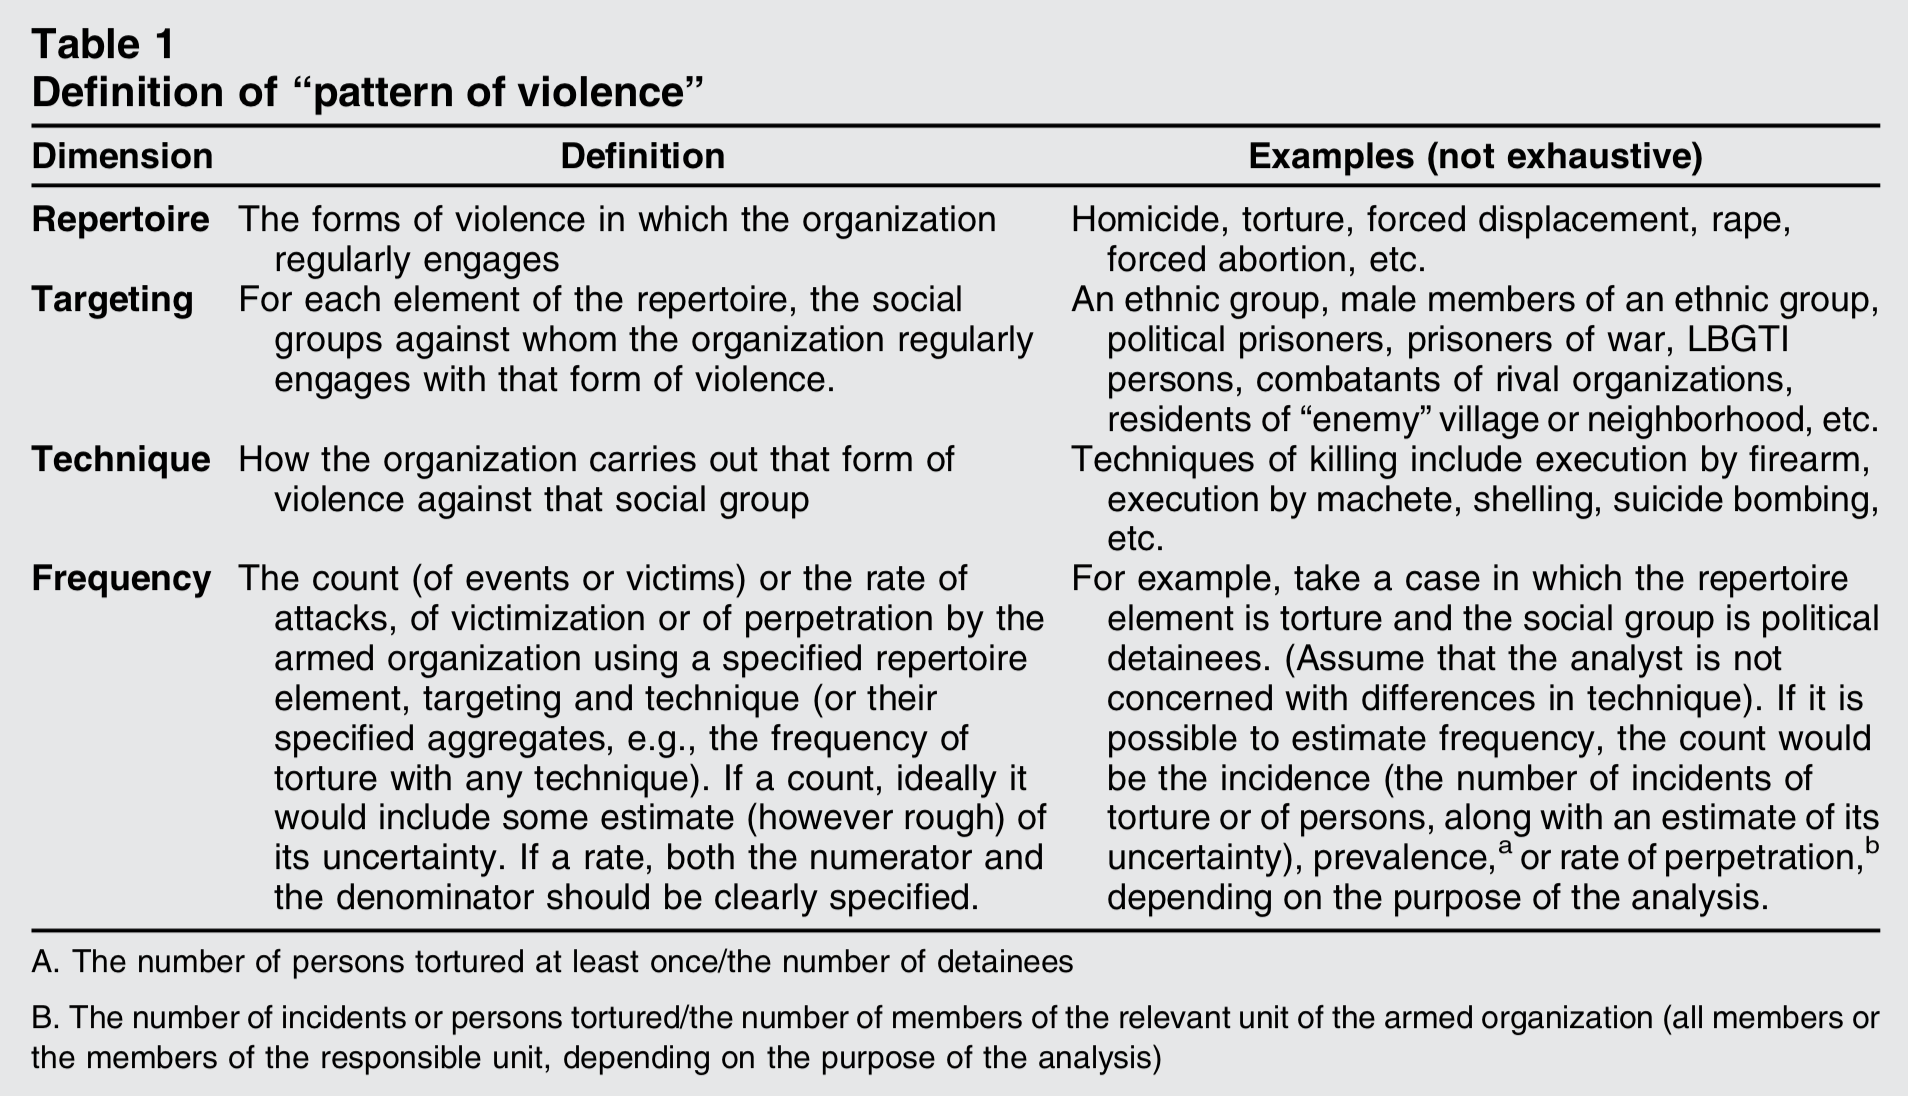
\includegraphics[width = 0.95\textwidth]{img/pattern_of_pv}

\vfill

\only<1>{
\begin{itemize}
  \item Applied to \BGyellow{armed groups} (rebels, states, etc)
\end{itemize}}

\only<2-3>{
\begin{itemize}
  \item For example, what's the pattern of \BGyellow<2>{Hamas}? \only<3>{\BGyellow<3>{FARC}?}
\end{itemize}}

\end{frame}
% ----------------------------------------------------

% ----------------------------------------------------
\begin{frame}
\frametitle{Patterns of political violence}
\centering

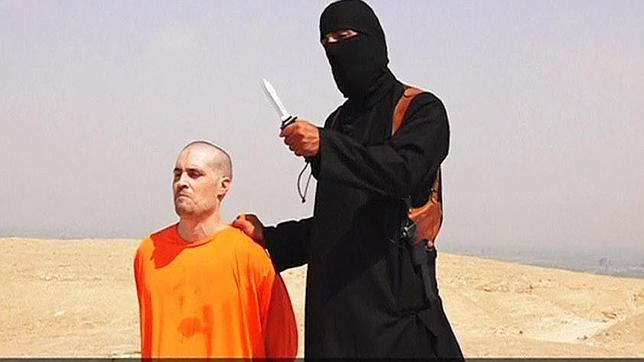
\includegraphics[width = \textwidth]{img/foley}

Sometimes groups are infamously famous for their repertoire

\end{frame}
% ----------------------------------------------------

% ----------------------------------------------------
\begin{frame}
\frametitle{Understanding violence against civilians}
\centering

\only<1>{\begin{itemize}
  \item Now the important question, why we observe civilian victimization?
\end{itemize}}

\only<2>{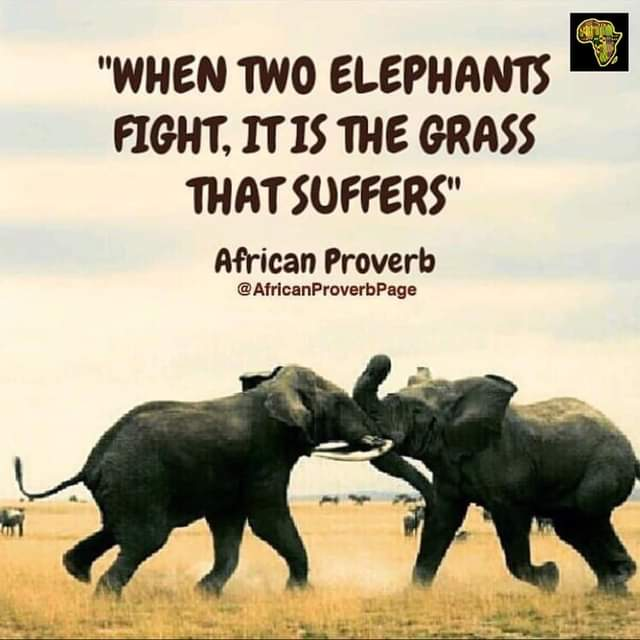
\includegraphics[width = 0.7\textwidth]{img/elephants}}

\only<3>{\begin{quote}
{\normalfont Lawrence Eagleburger (US Secr. of State) on Yugoslavia, in 1992:} ``this war is not rational. There is no rationality at all about ethnic conflict. It is gut, it is hatred; it’s not for any set of values or purposes; it just goes on''
\end{quote}}

\end{frame}
% ----------------------------------------------------

% ----------------------------------------------------
\begin{frame}
\frametitle{Understanding violence against civilians, pre 2000}
\centering

\begin{itemize}
  \item Violence against civilians seen as \BGyellow{collateral violence}
  \begin{itemize}
    \item Differences because of external factors: available weapons, population density, etc
  \end{itemize}
  \item
  \item When \textit{intentionality} could not be ignored (e.g. genocides, ethnic violence): \BGyellow{ancient hatreds}
\end{itemize}


\end{frame}
% ----------------------------------------------------

% ----------------------------------------------------
\begin{frame}
\frametitle{Understanding violence against civilians, pre 2000}
\centering

\begin{itemize}
  \item<1-> Problem with these perspectives? there's \textbf{nothing to explain}, violence happens because it happens
  \item[]
  \item<2->[] (There was an exception, actually: those who studied terrorism did view violence against civilians as instrumental)
\end{itemize}


\end{frame}
% ----------------------------------------------------

% ----------------------------------------------------
\begin{frame}
\frametitle{The new consensus}
\centering

\begin{itemize}[<+->]
  \item Problems:
  \begin{itemize}
    \item The ancient hatreds perspective is not useful: inter-ethnic violence is very rare even if ethnic tensions are common
    \item It's not only \textit{inter-}ethnic violence, also \textit{intra-}ethnic
    \item Previous `mass irrational violence' not useful either: most of the violence usually committed by a small percentage, often male linked to militias or paramilitary groups
  \end{itemize}
  \item Now we know that violence is an extension of war and an extension of politics
\end{itemize}



\end{frame}
% ----------------------------------------------------

% ----------------------------------------------------
\begin{frame}
\frametitle{Civilian killings and war}
\centering

\begin{itemize}
  \item<1-> Killing of civilians is deeply related to the central logic of the war
  \item<2-> Civilians are not bystanders to a war, they play a central role (offering support, human resources, etc) and, sometimes, they become the object of war
  \item<3-> Most attention on \textit{state-led} violence against civilians: because of their capacities (to inflict violence \& to control territory and have access to the civilian population), states have usually been the main perpetrators
  \begin{itemize}
    \item[] (Not always: ISIS' infamous record, West African rebel groups, ...)
  \end{itemize}
\end{itemize}

\end{frame}
% ----------------------------------------------------

% ----------------------------------------------------
\begin{frame}
\frametitle{Civilian killings and war}
\centering

\begin{itemize}
  \item<1-> Technology of rebellion and counter-insurgency strategy explain very well patterns of violence against civilians
  \item[]
  \item<2-> ``The guerrilla must move amongst the people as a fish swims in the sea'' (Mao Tse-Tung)
  \item<2-> Response by the state? General Ríos Montt in Guatemala: drain the sea in which the guerrilla swim
  \item<3-> More civilian victimization when state is uncapable of withdrawing support to the rebels or defeating them in some other way
  \item<3-> This logic easily leads to mass killing episodes, or ethnic cleansing in contexts whether support is assumed to follow ethnic lines
\end{itemize}

\end{frame}
% ----------------------------------------------------

% ----------------------------------------------------
\begin{frame}
\frametitle{Civilian killings and war}
\centering

\begin{itemize}
  \item<1-> Another perspective focuses on rebel groups and their incentives (rebel-led violence)
  \item<2-> Terrorism is a classic example: use of civilian killings to extract concessions from governments (particularly in democratic regimes, where people have more leverage)
  \item<3-> But rebel groups can also use violence to gain cooperation from civilians (typically, with territorial control)
  \begin{itemize}
    \item Weinstein 2007: if you depend on civilian cooperation for critical resources, you don't kill them, but if you extract your wealth from natural resources or external financing, you have less incentives not to kill
  \end{itemize}
\end{itemize}

\end{frame}
% ----------------------------------------------------

% ----------------------------------------------------
\begin{frame}
\frametitle{The politics of civilian killings}
\centering

\begin{itemize}
  \item<1-> Another point of view focuses on the political logic of victimization, which also applies to civilian killings \textit{outside} war
  \begin{itemize}
    \item What are the incentives of elites to engage in or promote violence against civilians?
  \end{itemize}
  \item[]
  \item<2-> Main idea: political elites obtain political benefits by promoting violence
  \begin{itemize}
    \item Does not necessarily lead to mass violence, but it can
  \end{itemize}
\end{itemize}

\end{frame}
% ----------------------------------------------------

% ----------------------------------------------------
\begin{frame}
\frametitle{The politics of civilian killings}
\centering

\begin{itemize}
  \item<1-> One example: ethnic outbidding
  \begin{itemize}
    \item I might gain political capital by being more radical than my competitors
    \item In a multi-ethnic context, this isn't usually good news
  \end{itemize}
  \item<2-> Role of ideology
  \begin{itemize}
    \item Sometimes seen as instrumental, but not so clear in other cases, e.g. anti-semitism in Nazi Germany, violence related to Communist agricultural policies, etc
    \item Ideology might play a bigger role as a \textit{restraining} factor
  \end{itemize}
  \item<3-> Getting away with violence
  \begin{itemize}
    \item Use more violence against opposition, media control, public cost vs private incentives, etc
  \end{itemize}
  \end{itemize}

\end{frame}
% ----------------------------------------------------


% ----------------------------------------------------
\begin{frame}
\frametitle{The microdynamics of civil wars}
\centering

\begin{itemize}[<+->]
  \item New type of studies after the mid-2000s: studying within-conflict dynamics, using micro-level data
  \item Quantitative analysis, archival data, case studies, etc
  \item Goal: know \textit{what} happened during a conflict and \textit{why} we see different levels of violence across different regions or municipalities
  \item (Problem? More difficult to generalize)
\end{itemize}

\end{frame}
% ----------------------------------------------------

% ----------------------------------------------------
\begin{frame}
\frametitle{The microdynamics of civil wars}
\centering

\begin{minipage}{0.59\textwidth}\centering
  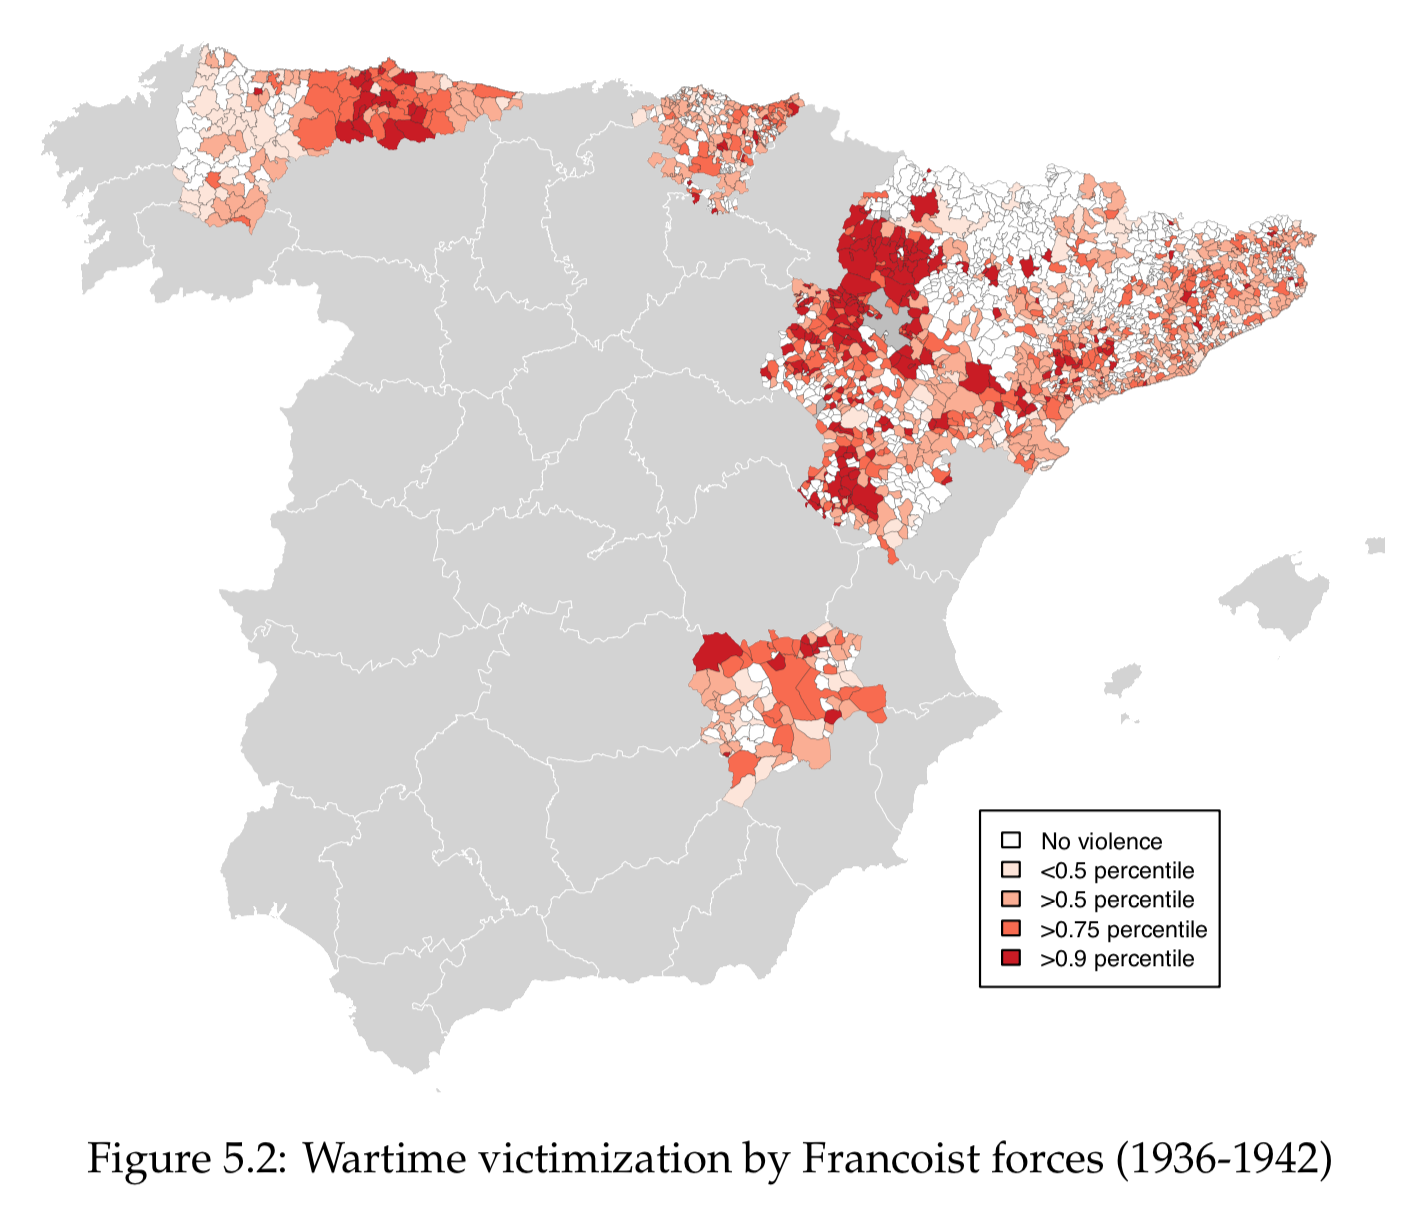
\includegraphics[width = \textwidth]{img/dissplot_spain}
\end{minipage}\hfill
\begin{minipage}{0.4\textwidth}\centering
  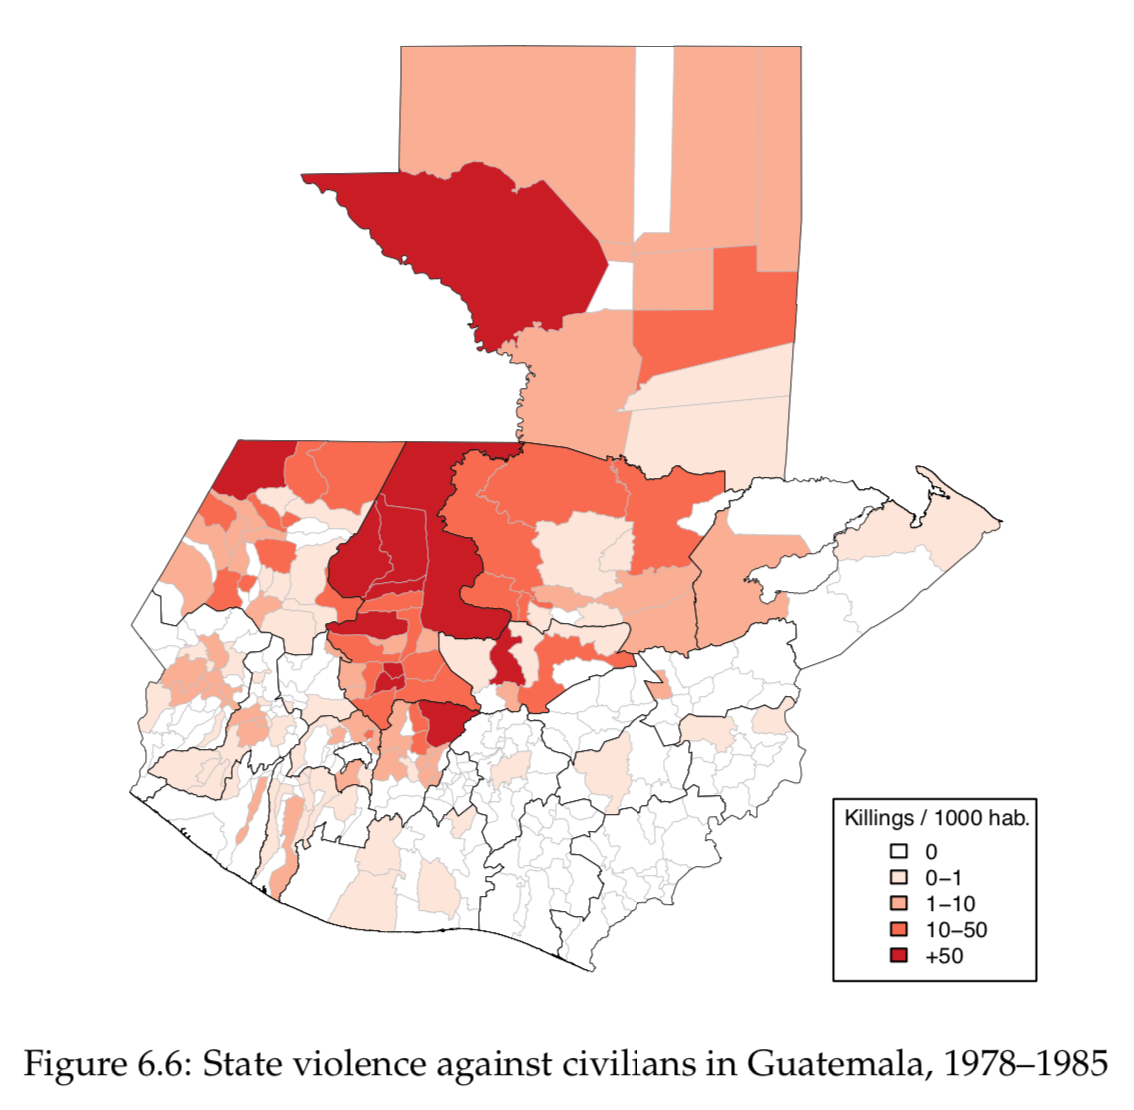
\includegraphics[width = \textwidth]{img/dissplot_guatemala}\\
  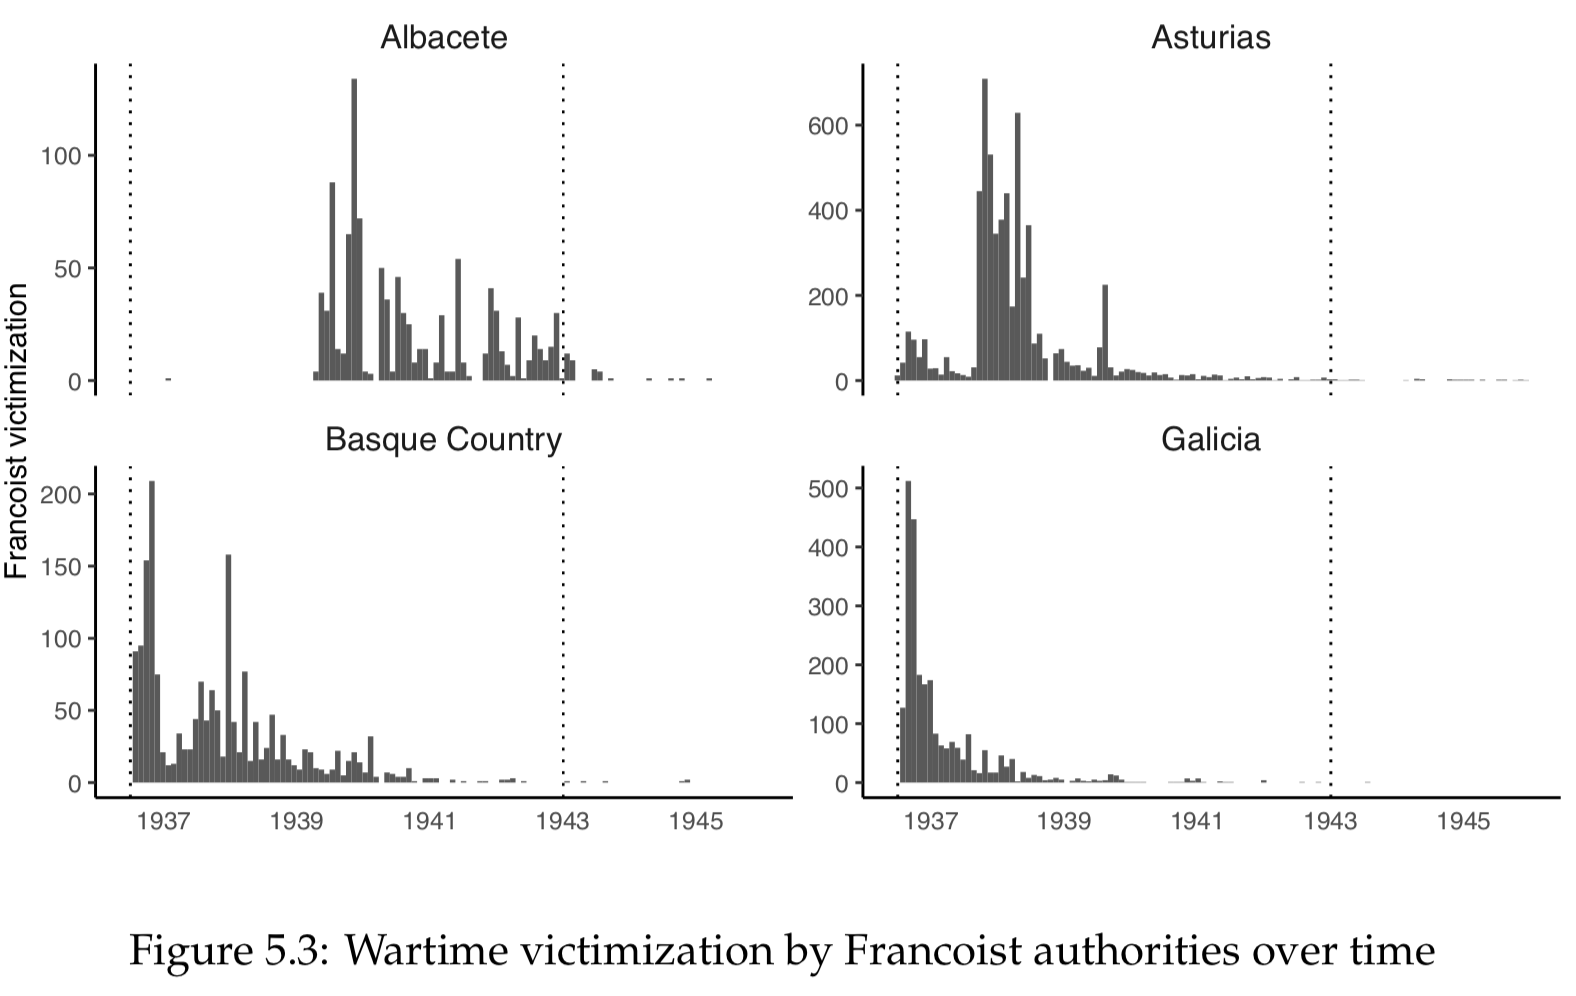
\includegraphics[width = \textwidth]{img/dissplot_time}
\end{minipage}

\end{frame}
% ----------------------------------------------------

% ----------------------------------------------------
\begin{frame}<1-3>[label=kalyvas]
\frametitle{The microdynamics of civil wars}
\centering

\begin{minipage}{0.69\textwidth}\centering
\begin{itemize}
  \item<2-> \textbf{Main idea}: violence is not about master cleavages, but about endogenous local conflicts motivated by \BGyellow{private reasons}: vendettas, local feuds, etc
  \item<3-> The setting: collaboration between local actors and external enforcers
  \begin{itemize}
    \item what do I gain or lose from collaborating with an armed actor? (e.g. rebels)
    \item and when do armed actors have incentives to use violence?
  \end{itemize}
  \item<4-> We should see more violence in areas where territorial control is not full
\end{itemize}
\end{minipage}\hfill
\begin{minipage}{0.3\textwidth}\centering
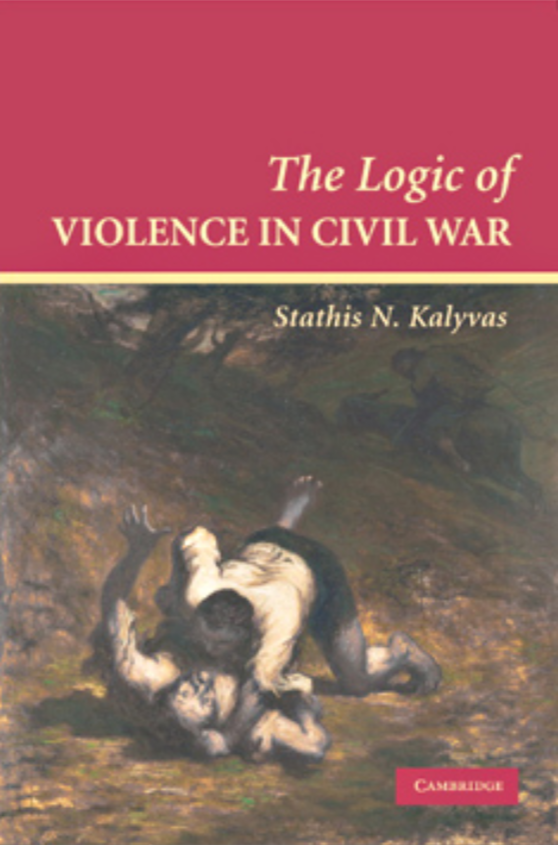
\includegraphics[width = \textwidth]{img/kalyvas2006}\\
{\footnotesize Stathis Kalyvas (2006)}
\end{minipage}

\end{frame}
% ----------------------------------------------------

% ----------------------------------------------------
\imageframe{img/kalyvas_model}
% ----------------------------------------------------

% ----------------------------------------------------
\imageframe{img/kalyvas_model2}
% ----------------------------------------------------

% ----------------------------------------------------
\againframe<4->{kalyvas}
% ----------------------------------------------------

% ----------------------------------------------------
\begin{frame}
\frametitle{Personal motives or politics?}
\centering

\begin{minipage}{0.49\textwidth}\centering
  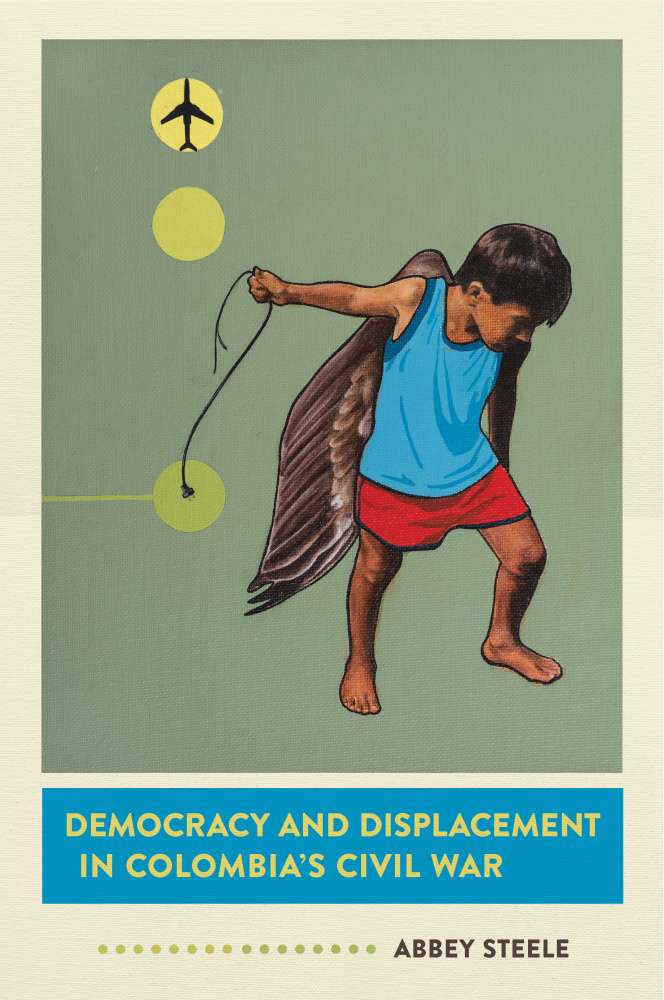
\includegraphics[width = 0.65\textwidth]{img/steele2017}\\
  {\footnotesize Abbey Steele (2017)}
\end{minipage}\hfill
\begin{minipage}{0.49\textwidth}\centering
  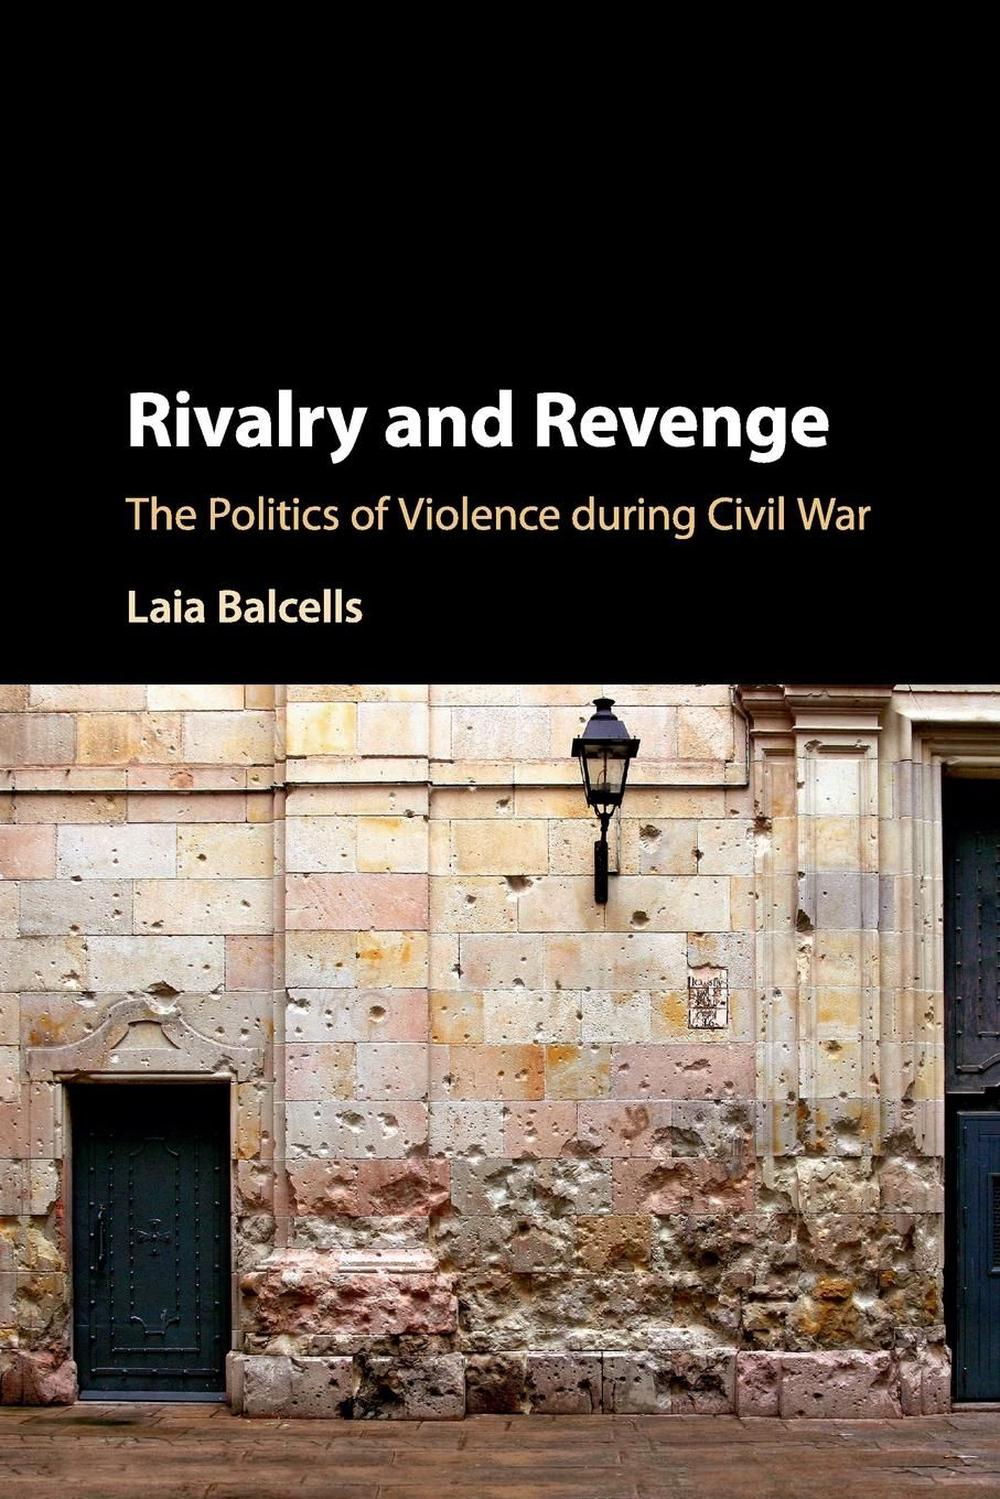
\includegraphics[width = 0.65\textwidth]{img/balcells2017}\\
  {\footnotesize Laia Balcells (2017)}
\end{minipage}

\vspace{10pt}

\begin{itemize}
  \item Two extensions to Kalyvas' model highlighting the role of \textit{political identity} in understanding wartime violence
\end{itemize}

\end{frame}
% ----------------------------------------------------

% ----------------------------------------------------
\begin{frame}
\frametitle{Personal motives or politics?}
\centering

\begin{itemize}
  \item<1-> Kalyvas' perspective emphasized that civil war violence emerges out of local grievances or feuds, private conflicts, vendettas, etc... and was \textit{later} interpreted along the master cleavage of the war
  \item<2-> But do political identities play a role?
  \item<2-> Think about the Spanish Civil War: is it that `reds' killed `blues' and vice-versa, or was violence produced by land disputes and enmities among neighbors who took advantage of the war to settle these conflicts?
\end{itemize}

\end{frame}
% ----------------------------------------------------


% ----------------------------------------------------
\begin{frame}
\frametitle{Personal motives or politics?}
\centering

\begin{itemize}
  \item Colombia: after elections were held, paramilitary groups could identify civilians perceived as loyal to the insurgents and implement political cleansing on those municipalities
  \item Spain: more \textit{direct} violence against civilians in those municipalities where electoral competition was higher, and a second round of violence motivated by revenge after territorial control changed
  \item Also in Spain: \textit{indirect} violence (e.g. bombings) directed at those areas that had politically supported the opposite side before the war
\end{itemize}

\end{frame}
% ----------------------------------------------------

% ----------------------------------------------------
\begin{frame}
\frametitle{Explaining killings}
\centering

\begin{itemize}
  \item The key idea is that killing civilians often responds to \textbf{strategic incentives}, not so much to irrationality
  \item The Q (or what changes from context to context) is about those incentives
  \item Understanding the structure of incentives helps understand most violence against civilians
  \begin{itemize}
    \item<2-> cases of \textit{irrational} violence?
  \end{itemize}
\end{itemize}

\end{frame}
% ----------------------------------------------------

% ----------------------------------------------------
\begin{frame}
\frametitle{Beyond fatal violence}
\centering

\begin{minipage}{0.65\textwidth}\centering
  \begin{itemize}[<+->]
    \item<2->[1.] Opportunistic rape
    \item<2->[] {\small (earlier perspective, anarchy during civil wars)}
    \item<3->[2.] Strategic violence
    \item<3->[] {\small (sowing fear, damaging the enemy, spoils of war, ...)}
    \item<4->[3.] Rape as a \BGyellow{practice}
    \item<5->[] e.g. Cohen (right): gang rape as a socialization practice within armed groups, more likely when there is \textit{forced recruitment}
  \end{itemize}
\end{minipage}\hfill
\begin{minipage}{0.34\textwidth}\centering
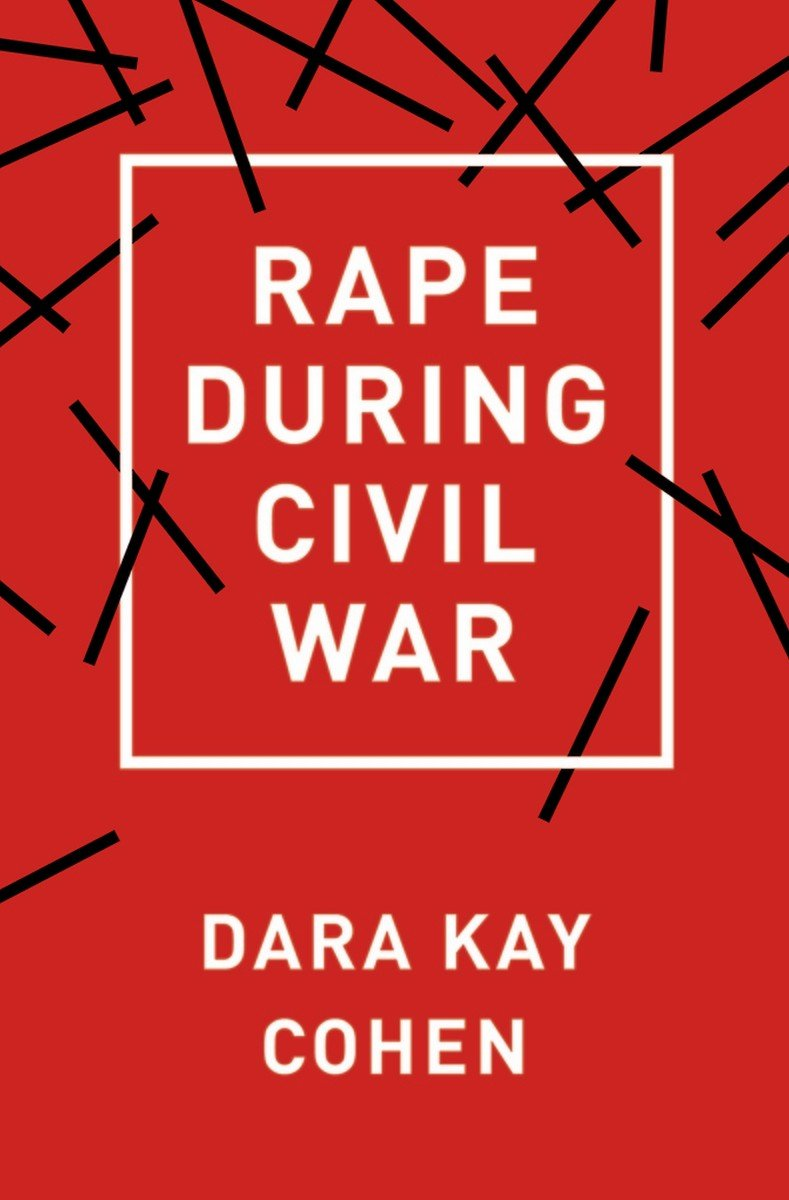
\includegraphics[width = 0.7\textwidth]{img/cohen_rape}\\Dara Kay Cohen (2016)
\end{minipage}

\end{frame}
% ----------------------------------------------------

% ----------------------------------------------------
\begin{frame}
\frametitle{Other examples from the Spanish civil war?}
\centering

\begin{itemize}
  \item Low-level internal purges and collective targeting
  \begin{itemize}
    \item Purges of schoolteachers \href{https://www.tandfonline.com/doi/abs/10.1080/13537113.2020.1795451}{\scriptsize (`The Double Logic of Internal Purges')}
  \end{itemize}
  \item Preemtive violence and local mobilizers
  \begin{itemize}
    \item Anticlerical violence %\href{}{\scriptsize (`Mobilization capacity and violence against local leaders')}
  \end{itemize}
\end{itemize}

\end{frame}
% ----------------------------------------------------

% ----------------------------------------------------
\begin{frame}
\frametitle{Zooming out: Why are civil wars so violent?}
\centering

\begin{itemize}
  \item[] Grand perspectives:
  \item[1.] \BGyellow<1>{Hobbessian anarchy}
  \begin{itemize}
    \item[] {\small (collapse of political authority)}
  \end{itemize}
  \item[2.] \BGyellow<2>{Transgression} (of the norms of war and violence)
  \begin{itemize}
    \item[] {\small (no rules apply during a war)}
  \end{itemize}
  \item[3.] \BGyellow<3>{Schmittian polarization}
  \begin{itemize}
    \item[] {\small (political or ethnic rivalry)}
  \end{itemize}
  \item[4.] \BGyellow<4>{Technology of warfare}
  \begin{itemize}
    \item[] {\small (explained by the way a civil war is fought)}
  \end{itemize}
\end{itemize}

\end{frame}
% ----------------------------------------------------

\end{document}
